\documentclass[11pt, a4paper]{article} %twoside
\usepackage{wrapfig}

\usepackage{epigraph}
\usepackage{graphicx}
\usepackage[swedish]{babel}

\usepackage[margin=3cm]{geometry}
\usepackage{float, blindtext, kantlipsum}
%\usepackage{multicol}

\usepackage[toc,page]{appendix}
\usepackage[section=subsection, toc, acronym, nonumberlist]{glossaries}
\renewcommand{\appendixtocname}{Bilagor} \renewcommand{\appendixpagename}{Bilagor}
\addto\captionsswedish{\renewcommand\appendixname{Bilagor}}

%\renewcommand{\thefootnote}{\alph{footnote}}

\newcommand{\symfootnote}[1]{%
\let\oldthefootnote=\thefootnote%
\stepcounter{mpfootnote}%
\addtocounter{footnote}{-1}%
\renewcommand{\thefootnote}{$\dagger$}%
\footnote{#1}%
\let\thefootnote=\oldthefootnote%
}

\usepackage[citestyle=verbose-ibid, bibstyle=authoryear, natbib=true, url=false, doi=false, isbn=false, backend=biber, labeldateparts]{biblatex}
\AtEveryBibitem{%
  \clearlist{language}%
  \clearfield{note}%
}
%\DeclareBibliographyDriver{misc}{%
%  \usebibmacro{bibindex}%
%  \usebibmacro{begentry}%
%  \printfield{author}%
%  \setunit{\labelnamepunct}\newblock
%  \usebibmacro{maintitle+title}%
%  \newunit
%  \usebibmacro{date}%
%  \newunit\newblock
%  \printfield{number}%
%  \newunit
%  %\usebibmacro{byeditor+others}%
%  \setunit{=\addspace}
%  \printfield{series}%
%  \setunit{\adddot\addspace}
%  \usebibmacro{publisher+location+date}%
%  \newunit\newblock
%  \usebibmacro{finentry}}
%
\DeclareBibliographyDriver{audio}{%
  \usebibmacro{bibindex}%
  \usebibmacro{begentry}%
  \printfield{usera}%
  \setunit{\labelnamepunct}\newblock
  \usebibmacro{maintitle+title}%
  \newunit
  \usebibmacro{date}%
  \newunit\newblock
  \printfield{number}%
  \newunit
  %\usebibmacro{byeditor+others}%
  \setunit{=\addspace}
  \printfield{series}%
  \setunit{\adddot\addspace}
  \usebibmacro{publisher+location+date}%
  \newunit\newblock
  \usebibmacro{finentry}}
%\usepackage{hyperref}
\addbibresource{bibtex/kandidatarbete.bib}

\usepackage{csquotes}

\usepackage{sectsty}
\subsubsectionfont{\normalfont\itshape}
%\subsectionfont{\normalfont\centering}

\usepackage{titlesec}
\titleformat{\section}
  {\normalfont\LARGE\bfseries}{\thesection}{1em}{}[{}]

  \newcommand{\sectionbreak}{\clearpage}
  %\titlerule[0.8pt]

\makeglossaries

\newacronym{api}{API}{Application Programming Interface}
\newacronym{cgm}{CGM}{Continuous Glucose Monitor}
\newacronym{fgm}{FGM}{Flash Glucose Monitor}
\newacronym{pmson}{PMSon}{Parameter Mapping Sonification}
\newacronym{fifo}{FIFO}{First In, First Out}

\setglossarystyle{long}

%\newglossaryentry{API}
%{
%    name=API,
%	description={Application Programming Interface.}
%}


\newglossaryentry{frontend}
{
    name=Front end,
	description={Användargränssnittet i webbutveckling}
}

\newglossaryentry{backend}
{
    name=Back end,
	description={Allt som rör sig ''under huven'', server-side programmering}
}

\newglossaryentry{supercollider}
{
    name=SuperCollider,
	description={Ett programmeringsspråk och plattform för syntes av ljud, och musikalisk programmering}
}

\newglossaryentry{pattern}
{
    name=Pattern,
	description={Ett verktyg i SuperCollider för att generera ...}
}

\newglossaryentry{stack}
{
    name=Stack,
	description={Alla delar som utgör en plattform eller ett system. Finns olika vanligt använda}
}

\newglossaryentry{audification}
{
    name=Audifiering,
	description={en. \emph{audification}. Att direktöversätta en dataserie till ljudkurvor}
}

%\newglossaryentry{fifo}
%{
%    name=FIFO-system,
%	description={First in, First out. En typ av kösystem}
%}

\newglossaryentry{sonification}
{
    name=Sonifiering,
	description={en. \emph{sonification}. Att översätta en dataserie}
}

\newglossaryentry{mappning}
{
    name=Mappning,
	description={eller \emph{avbildning}. Ihopparningen av ett element (invariabel) till en annan (utvariabel). Olika typer av mappningar finns, till exempel \emph{injektiv} eller \emph{one-to-one}}
}

\newglossaryentry{parametermapping}
{
    name=Parameter Mapping Sonification,
	description={}
}
\begin{document}

\clearpage


\newpage
%\begin{multicols}{2}

\renewcommand{\abstractname}{Tack}
\begin{abstract}
  Stort tack till min texthandledare Kim Hedås och lärare Erik Peters för alla kloka råd och vägledning! Även stort tack till Herman Wikner\symfootnote{Hermans GitHub finns tillgänglig på: \url{https://github.com/hermanwikner} (hämtad \today).} som hjälpt mig bygga användargränssnittet i React! 
\end{abstract}
\tableofcontents

\section*{Introduktion}
\addcontentsline{toc}{section}{Introduktion}
Denna text kompletterar mitt examensprojekt, \emph{Radio Diabetes}, en interaktiv komposition/installation som generarar musik av blodsockervärden. Installationen består av ett SuperCollider\footcite{noauthor_supercollider_nodate}-program som skapar själva musiken och en webbplats där man kan lyssna på den, läsa om projektet och ladda upp sina egna blodsockervärden. När en deltagare laddar upp sina värden slussas dessa direkt vidare till SuperCollider-programmet, som i sin tur inkluderar dem i musiken, antingen direkt eller att de blir schemalagda i en kö. Musiken strömmas till webbplatsen (och vidare till lyssnaren) via en internetradiostation. På så sätt utgör musiken ett kontinuerligt flöde som deltagare och åhörare hör samtidigt: det finns ingen början, mitten eller slut, utan endast ett \emph{nu}. %Denna förhållning till \emph{temporalitet} utgör ett huvudtema i projektet, jämte med \emph{interaktivitet} (deltagande), \emph{radioteknologi}, \emph{autoimmuna sjukdomar} och \emph{sonifiering}.

% TODO minska antalet "huvudteman"...?!
% TODO "tystnad i radio"
%\emph{(I skrivande stund är installationen inte helt färdig.)}


\subsection*{Bakgrund}
\addcontentsline{toc}{subsection}{Bakgrund}
Idéen om att göra musik av blodsockervärden föddes dagen då jag fick en \emph{Freestyle Libre}-mätare, en så kallad kontinuerlig blodsockermätare, eller \gls{cgm}. Denna typ av blodsockermätare skiljer sig från tradionella mätare --- som man är tvungen att sticka sig i fingret och på så sätt mäta blodsockret med --- i att den regelbundet gör mätningar, vilket ger en kontinuerlig kurva över ens blodsockervärden. Kurvorna påminde mig om hur ljudsignaler ofta representeras visuellt (en horisontell tidsaxel och en linjär vertikal axel) och i ett tidigt experiment gjorde jag en direkt översättning av mina blodsockerkurvor till ljudfiler: en så kallad \emph{audifiering}. Dessa ljud använde jag som samplingar i mitt stycke \emph{Värden och en vagga} (2017), som var ett av arbetsproverna jag sökte till Musikhögskolan med. 

Jag utvecklade vidare och förbättrade mitt första program som jag hade skrivit för att översätta mina kurvor till ljudfiler, så att vem som helst skulle kunna använda programmet och översätta sina enga värden till ljud. Jag byggde också en wavetable-synth i SuperCollider som använde dessa ljudfiler som källmaterial. Detta instrument har jag använt i ett antal olika kompositioner som jag skrivit under min skoltid. Båda dessa program (översättaren och wavetable-synthen) har jag publicerat på min Github\footcite{jondell_kj-jondelldiabetes-synth_2021}. En del av denna kod återanvände jag även i detta projekt.

\subsection*{Några tidigare exempel, historiska och nutida}
\addcontentsline{toc}{subsection}{Några tidigare exempel, historiska och nutida}
Här har jag valt ut ett par exempel av musik och ljudinstallationer komponerad utifrån biologiska signaler och mätvärden för att ge ett historiskt perspektiv och nutida sammanhang.

Alvin Lucier bör anses som en pionjär inom detta fält, då han redan 1965 skrev stycket \emph{Music for Solo Performer}\footcite{lucier_music_1965}. I detta verk låter han uppmäta alfavågor med elektroder kopplade till huvudet av interpreten/utövaren. Dessa vågor förstärks sedan och spelas upp i 16 högtalare, som i sin tur exiterar diverse slagverk. Lucier kommenterade om stycket, i ett seminarium 2001 citerat av Straebel och Thoben\footcite{straebel_alvin_2014}:

\begin{quote}
  I thought, 'I don't have a structure for this.' I mean, I'm a composer. I should impose some kind of structure, but then I thought, no, brain waves are a natural phenomen. They should just flow out ... 
\end{quote}

Detta belyser Luciers generativa förhållande till formen, och den direkta kopplingen mellan den uppmätta signalen och ljudvågorna är ett tidigt exempel på \emph{audifiering}.

På senare tid har ett antal genrer eller rörelser uppkommit med utgångspunkt i sonifieringen av biologisk data, med namn som \emph{protein music}\footcite{king_pm_1996}, \emph{DNA music}\footcite{k_kawazoe_study_2001} och \emph{gene music}\footcite{munakata_gene_1995}. Dessa genrer utgår samtliga från att låta musiken styras av dataset bestående av DNA-sekvenser, protein eller gener, till exempel mappningen av kvävebaser till tonhöjd\footcite{shi_electronic_2007}. Det finns ett visst vetenskapligt anspråk i de texter som skrivs om dessa olika typer av musik, att sonifieringen kan ge en typ av insikt i de dataset som används som en visualisering \emph{inte} skulle ge\footcite{king_pm_1996}. Detta anspråk har dock nyanserats och kritiserats på senare tid, av till exempel forskaren och kompositören Peter E. Larsen\footcite{larsen_more_2016} som menar att sonifieringen knappast leder till någon djupare insikt än ett vanligt stapeldiagram. Jag vill lyfta Dr. David Deamers och Riley McLaughlins \emph{Insulin A \& B Chains} (1983)\footcite{deamer_insulin_1983} och Dr. Nobuo Munakatas \emph{Hugging Tightly: Human RNase Inhibitor} (2009)\footcite{munakata_hugging_2009} som två nämnvärda exempel av \emph{DNA}, eller \emph{protein music}, som jag inspirerats av rent estetiskt.

Den 2 april 2021 släpptes Luca Yupanquis album \emph{Sounds of the Unborn}\footcite{yupanqui_sounds_2021}, som spelades in redan innan hon var född. Yupanquis föräldrar --- musikerna Elizabeth Hart och Iván Diaz Mathé --- hade med hjälp av elektroder kopplade till Harts kropp spelat in deras ofödda barns \emph{in utero}-rörelser och sedan låtit sonifiera dessa inspelade signaler med ett system utvecklat av Sam Cusumano och hans företag \emph{Electricity for progress}\footcite{noauthor_electricity_nodate}. Elizabeth Hart berättar i en intervju i \emph{Kulturnytt i P1}\footcite{eklund_duo_2021} hur musiken kommit till av ett rent experimenterande, att föräldrarna till en början inte hade haft en tanke att ge ut det som ett album. Hart berättar vidare att hon \textbf{inte} tror att musiken säger något speciellt om de ofödda, att det inte varit föräldrarnas avsikt, och avfärdar frågan om huruvida processen endast varit ett PR-trick med att säga: ''... for us, I think it is a pretty great album. Musically, I am proud of what was achieved, musically.'' Skivbolaget \emph{Sacred Bones Records}, som släppt albumet, säljer systemet som Hart och Diaz Mathé använt under namnet \emph{MIDI Biodata Sonification Device}\footcite{noauthor_midi_nodate} och Cusumano, som utvecklat systemet, driver ett forum\footcite{noauthor_biodata_nodate} där användare av detta system uppmuntras dela med sig av olika sonifieringar de gjort. 


\emph{r a d i o q u a l i a} är ett kollektiv bestående av de två nya zeeländska konstnärerna Honor Hargar och Adam Hyde som utforskar användandet av radio och internetradio som konstmedium\footcite{noauthor_r_nodate}. Hargar och Hyde startade samarbetet 1998 och har gjort projekt som bland annat \emph{Free Radio Linux}\footcite{r_a_d_i_o_q_u_a_l_i_a_free_2002} --- en radioutsänd  (både marksänd och via internetradio) datoriserad uppläsning av de fyra miljoner rader kod som Linux operativsystemskärna då bestod av, med start den 3e februari 2002 --- och \emph{Radio Astronomy}, en sonifiering/audifiering av signaler uppmätta med ett radioteleskop, som i realtid utsänds dels via AM, FM och kortvågsradio, dels via konstnärernas hemsida. I en text\footcite{perron_radioqualia_2003} av Jacques Perron som behandlar just \emph{Radio Astronomy} citeras den tyska dramatikern Berolt Brecht, som i sin text \emph{The Radio as an Apparatus of Communication}\footcite{brecht_radio_nodate} från 1927 skrev:
\begin{quote}
  Radio is one sided when it should be two. It is purely an apparatus for distribution, for mere sharing out. So here is a positive suggestion: change this apparatus over from distribution to communication. The radio would be the finest possible communication apparatus in public life, a vast network of pipes. That is to say, it would be if it knew how to receive as well as transmit, how to let the listener speak as well as hear, how to bring him into a relationship instead of isolating him. On this principle the radio should step out of the supply business and organise its listeners as suppliers.
\end{quote}
%Interaktivitet (\emph{Calling out of context})...


%Radio (\emph{Tuning a radio}, etc...)
\subsection*{Radio}
\addcontentsline{toc}{subsection}{Radio}
En del av installationen består av en internetradiostation, som strömmar ut den genererade musiken. Radion som medium påverkar i hög grad själva innehållet, det vill säga musiken, i olika avseenden, till exempel dess temporalitet och interaktivitet. 
Marshall McLuhan beskriver i sin bok \emph{Understanding media: the extensions of man}\footcite{mcluhan_understanding_2003} radion som ett \emph{hot medium}\footcite[39]{mcluhan_understanding_2003}, något han menar är ett medium som ''...extends one single sense in '\emph{high definition}'... the state of being well filled with data.'', men som följdaktligen inte ger mycket utrymme för deltagande. McLuhan kontrasterar detta med exempel av \emph{cool media} som telefonen, där innehållet skapas helt av deltagarna (\emph{high} och \emph{low definition} ska alltså inte blandas ihop med ljudkvalitet i detta fall). Den första utgåvan av \emph{Understanding media} kom 1964, en tid då dessa medier kanske var mer kategoriskt \emph{hot} eller \emph{cool}. I Jonas Anghammars C-uppsats \emph{Nya medier möter gamla radion: publikmedverkan i public service-radion nu och då}\footcite{anghammar_nya_2010} från 2010 går det att läsa om hur graden av interaktion i Svergies Radios programutbud ökat markant bara sedan 90-talet, något som kopplas samman med den snabba digitaliseringen som skett. Anghammars skriver i ett citat av Nils Enlund från 2008 att ''...publiken nu själva skapar stor del av medieinnehållet eftersom den tillåts göra det.'' Kanske undergår radion, som medium, en nedkylning. En del i utvecklingen av förgörelsen av tid och rum som McLuhan menar elektrifieringen av vår värld har påkallat: ''With instant electric technology, the globe itself can never again be more than a village...''\footcite[454]{mcluhan_understanding_2003}.

%Jämförelsevis så är \emph{Ring så spelar vi}, \emph{Karlavagnen} och \emph{Ring P1} exempel på program i traditionell marksänd rundradio som består av en hög grad av deltagande, eller interaktivitet. Dessa bygger i princip helt på att lyssnare ringer in och innehållet skapas av lyssnardeltagandet. 

%Radion som konstmedium har länge inspirerat mig, från hörspelen av bland andra Öyvind Fahlström, till John Cages radiokompositioner, till mer sentida \emph{radioqualia}... 

%Hot/cool media (McLuhan), interaktion, 

%''Ring så spelar vi'' och ''Ring P1'' är två exempel på interaktiva radioprogram, där lyssnarna till hög grad styr och påverkar programmets innehåll. I "Ring P1", som sänds live, är interaktionen så hög att diskussioner kan uppstå lyssnare emellan, där en lyssnare replikerar en annan lyssnares inlägg eller deltagande. Men trots denna höga grad av fri interaktion behöver varje deltagare först passera en telefonsluss. 

%Digital mediekonst som bygger kring internetradio, eller så kallad \emph{streaming culture}, 
%använder sonifieringar

% \emph{r a d i o q u a l i a}...
\subsection*{Sonifiering}
\addcontentsline{toc}{subsection}{Sonifiering}

I det andra kapitlet av antalogin \emph{The Sonification Handbook}, skrivet av Walker och Nees\footcite[9]{hermann_theory_2011}, ges en möjlig definition av  \gls{sonification} som användandet av icke-tal ljud för att presentera/representera information, eller mer specifikt översättningen av förhållanden i information till ljud som gör dessa förståeliga för oss, tack vare våra hörsystem. Som tidigare nämnt görs ofta ett vetenskapligt anspråk i användandet av sonifiering något med potential att ge åhörare i allmänhet, och forskare i synnerhet, en insikt\footnote{\emph{Insikt} som ord är något ironiskt ett bra exempel på hur invand användningen av visuell representation är för \emph{förståelsen}.} som en annan representation av informationen inte hade gett, eller kunnat ge.  

I detta projekt tar jag avstånd från idéen om att användandet av \emph{sonifiering} på något sätt ska skänka insikt till datan som jag låter gestalta i musiken: tvärtom hoppas jag att den musikaliska gestaltningen \emph{inte} kommer avslöja något om de bakomliggande mätvärdena. Jag kommer trots det göra en kortare sammanfattning av olika \emph{sonifieringstekniker- } och \emph{kategorier} som redogörs i \emph{The Sonification Handbook}, för att sätta ord på det jag har gjort i detta projekt.% (fastän ändamålet inte varit detsamma som föreslås i antalogin). % och som senare tillåter en tydligare diskussion av resultaten.




%Sonifiering (eller är det verkligen sonifiering). %\footcite[2]{bijsterveld_sonic_2019}
%Smalley och spektromorfologin. \footnote{Olika ordningar av \emph{surrogacy},  gestaltandet av \emph{datan}.} Bearbetad data och orginaldata. Sensorfel.

%Parameter Mapping Sonification (PMSon)
%\gls{mappning}
%
%\gls{audification} \footcite[302]{hermann_audification_2011} är en form av sonifiering där mätdatan översätts direkt till ljudkurvor... fyra grupper av data (\emph{sound recording}, \emph{general acoustic}, \emph{physical}, och \textbf{\emph{abstract}})...
%

\subsection*{Diabetes}
\addcontentsline{toc}{subsection}{Diabetes}

Diabetes mellitus är en auto-immun sjukdom som huvudsakligen finns i två olika varianter: typ-1 diabetes och typ-2 diabetes. Insulinproduktion/insulinresistens. I Sverige finns x antal typ 1-diabetiker, och i världen (siffra). Jag debuterade (en? två? tre?) veckor efter jag hade börjat ettan i grundskolan, hösten 2001. Sedan dess har jag dagligen tagit insulininjektioner och mätt mitt blodsocker, inför varje måltid och däremellan. Jag har haft otaliga episoder av lågt och högt blodsocker (hypo- och hypoglycemi). Som diabetiker kan j Sjukdomen är kronisk.


\subsubsection*{Blodsockervärden}
\addcontentsline{toc}{subsubsection}{\textit{Blodsockervärden}}
Blodsocker mäts i mmol/L och varierar hos en icke-diabetiker mellan 4 och 6 mmol/L [källa]. Hos en diabetiker kan detta värde variera från under 1 till över 30 mmol/L, och Freestyle Libre-sensorn har ett spann på att mäta från lägst 2,2 till 27,7 mmol/L (annars visar den \emph{LO} respektive \emph{HI}). Freestyle Libre-sensorn mäter kontinuerligt var 15:e minut.

%Att s.k. \emph{mappa} denna data till musikaliska parametrar är förstås godtyckligt --- värdena i sig har ingen musikalisk mening --- och bör så vara: det är helt enkelt mina konstnärliga val som bestämmer hur de förhåller sig till varandra. Även en bearbetad signal går att använda för att styra musiken: interpolation (mellan de diskreta mätpunkterna), variation (FFT, derivator, etc.), stokastiska egenskaper (auto-korrelation etc), statistiska egenskaper (median, medel, etc.). ''\emph{Tid i målområdet}'' och liknande värden kan också vara intressanta att använda, och har medicinsk betydelse.

%Det som är viktigt i denna \emph{mappning} är dock att den gestaltade datan --- dvs. musiken --- \textbf{inte} får avslöja något om den underliggande eller bakomliggande (mät)datan. Dels är det en integritetsfråga, som diskuteras vidare nedan, dels är det en förutsättning för detta projekt: det existerar inga \emph{bra} eller \emph{dåliga} värden. Själva delningen av värdena är det viktiga.

\subsubsection*{Förhållandet till mätandet}
\addcontentsline{toc}{subsubsection}{\textit{Förhållandet till mätandet}}
I sin text \emph{Det autoimmuna jaget --- om att sätta gränser} \footcite[286]{arvidson_det_2016} skriver Mats Arvidson om kravet som diabetiker på disciplin \emph{och} prestation.

Prestation, utmattning (bornemark...utmattning...)? Krav och värden... 

Ett sentiment som ofta förekommande (''jag är \textbf{inte} min diabetes, mina blodsockervärden...'', t.ex. artikel i \emph{Hälsoportalen}(???))

\subsection*{Datainsamling}
\addcontentsline{toc}{subsection}{Datainsamling}
Eftersom detta projekt beror av insamling av biometrisk data, som enligt \emph{Dataskyddsförordningen} (GDPR) \footcite{integritetsskyddsmyndigheten_kansliga_nodate} är en känslig personuppgift, krävs ett uttryckligt samtycke från varje deltagare att denna är införstådd i hur datan behandlas. Jag har försökt vara så transparent som möjligt i hur datan behandlas, genom att dels dela \textbf{all} källkod som jag använder, och även i den kommunikation jag lagt ut på webbplatsen och i övriga dokument berörande projektet (såsom denna text). All data som samlas in anonymiseras/avidentifieras så fort som möjligt och den är inte sparad någonstans utöver arbetsminnet som SuperCollider använder. I enlighet med Vetenskapsrådets text \emph{God forskningssed} \footcite[s. 40-41]{vetenskapsradet_god_2017} är sekretess, anonymitet och integritet av största vikt i detta projekt, även fast det är ett konstprojekt och inte ett forskningsprojekt. Jag har inget kommersiellt intresse i insamlingen av datan, jag delar den inte med någon extern part heller, och allt deltagande är valfritt. Min ambition är \textbf{inte} att samla data för sakens skull, utan att diabetiker ska kunna dela med sig av sina värden utan att de på något sätt bedöms eller värderas: helt enkelt, att själva delandet och deltagandet i sig står i fokus. 

\section*{Process}
\addcontentsline{toc}{section}{Process}
Installationen består som tidigare nämnt av två delar: ett musikgenererande program (SuperCollider) och en webbplats (se figur \ref{hemsida} på nästa sida). Här nedan följer en teknisk beskrivning av detta system.

\begin{figure}[H]
\centering
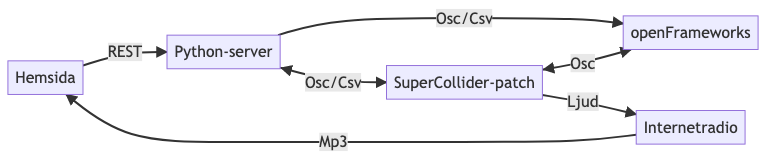
\includegraphics[width=0.5\textwidth]{../media/flowchart.png}
\caption{Översiktsdiagram av system}
\end{figure}


\subsection*{SuperCollider-system}
\addcontentsline{toc}{subsection}{SuperCollider-system}
% TODO LÄGG TILL ETT BLOCKDIAGRAM SOM ILLUSTRERAR SUPERCOLLIDER SYSTEMET
När en deltagare laddar upp en fil med sina mätvärden så skickas de vidare, via Python-servern, till \gls{supercollider}-programmet, som spelar upp en tack-hälsning för att ge en direkt återkoppling till deltagandet. Varje instans av mätdata --- det vill säga varje bidrag till, eller varje interaktion med, installationen --- gestaltas av en specifik musikalisk funktion, för att på sätt ge deltagaren en koppling och förståelse till hur dennes bidrag påverkar musiken. Till exempel kan ett uppladdat paket av data ge upphov till ett arpeggio, någon form av melodi eller en underliggande ljudmatta. I SuperCollider-programmet representeras varje sådan instans av mätdata av ett \emph{objekt}, som innehåller attribut som bland annat: register, skala, speltid, panorering, klangkälla/\emph{SynthDef}, och tillhörande \emph{\gls{pattern}}. Dessa attribut är antingen direkt bestämda av mätdatan (en så kallad \emph{mappning}) eller bestämda utifrån de andra aktiva objekten, till exempel förhåller de sig till redan ''upptagna'' register. Skapandet av dessa objekt gör programmet så fort det mottagit ett nytt paket av mätdata från Python-servern. Samtidigt avgör programmet om objektet ska spelas upp direkt, eller om det ska läggas på kö. 

\subsubsection*{Kösystemet}
\addcontentsline{toc}{subsubsection}{\emph{Kösystemet}}
Behovet av ett kösystem kommer ur scenariot att flera deltagare laddar upp värden inom en relativt kort tidsram. Om detta händer \emph{utan ett kösystem}, kan systemet reagera på två sätt: antingen spelas alla objekt upp samtidigt, med risk för att överrösta varandra och bli en kakofoni, eller så ersätter de varandra, vilket skulle leda till att ens bidrag inte skulle höras mer än en väldigt kort stund. En kompromiss är att använda ett kösystem, så att antalet samtidigt spelande objekt begränsas, och att dessa spelas \emph{minst} en given längd tid, men inte längre än en annan bestämd tid, om det står väntande deltagare på kö. Allt som allt har jag begränsat antalet samtidigt spelande objekt till \emph{tre} stycken, och när dessa är fyllda ställs antingen ett nytt bidrag på kö --- om inte de spelande objekten har varit aktiva i den givna minimumtiden --- eller så ersätter det nya bidraget det äldsta spelande objektet. Kösystemet är i tekniska termer alltså ett \gls{fifo}-system.

\begin{figure*}[ht!]
\centering
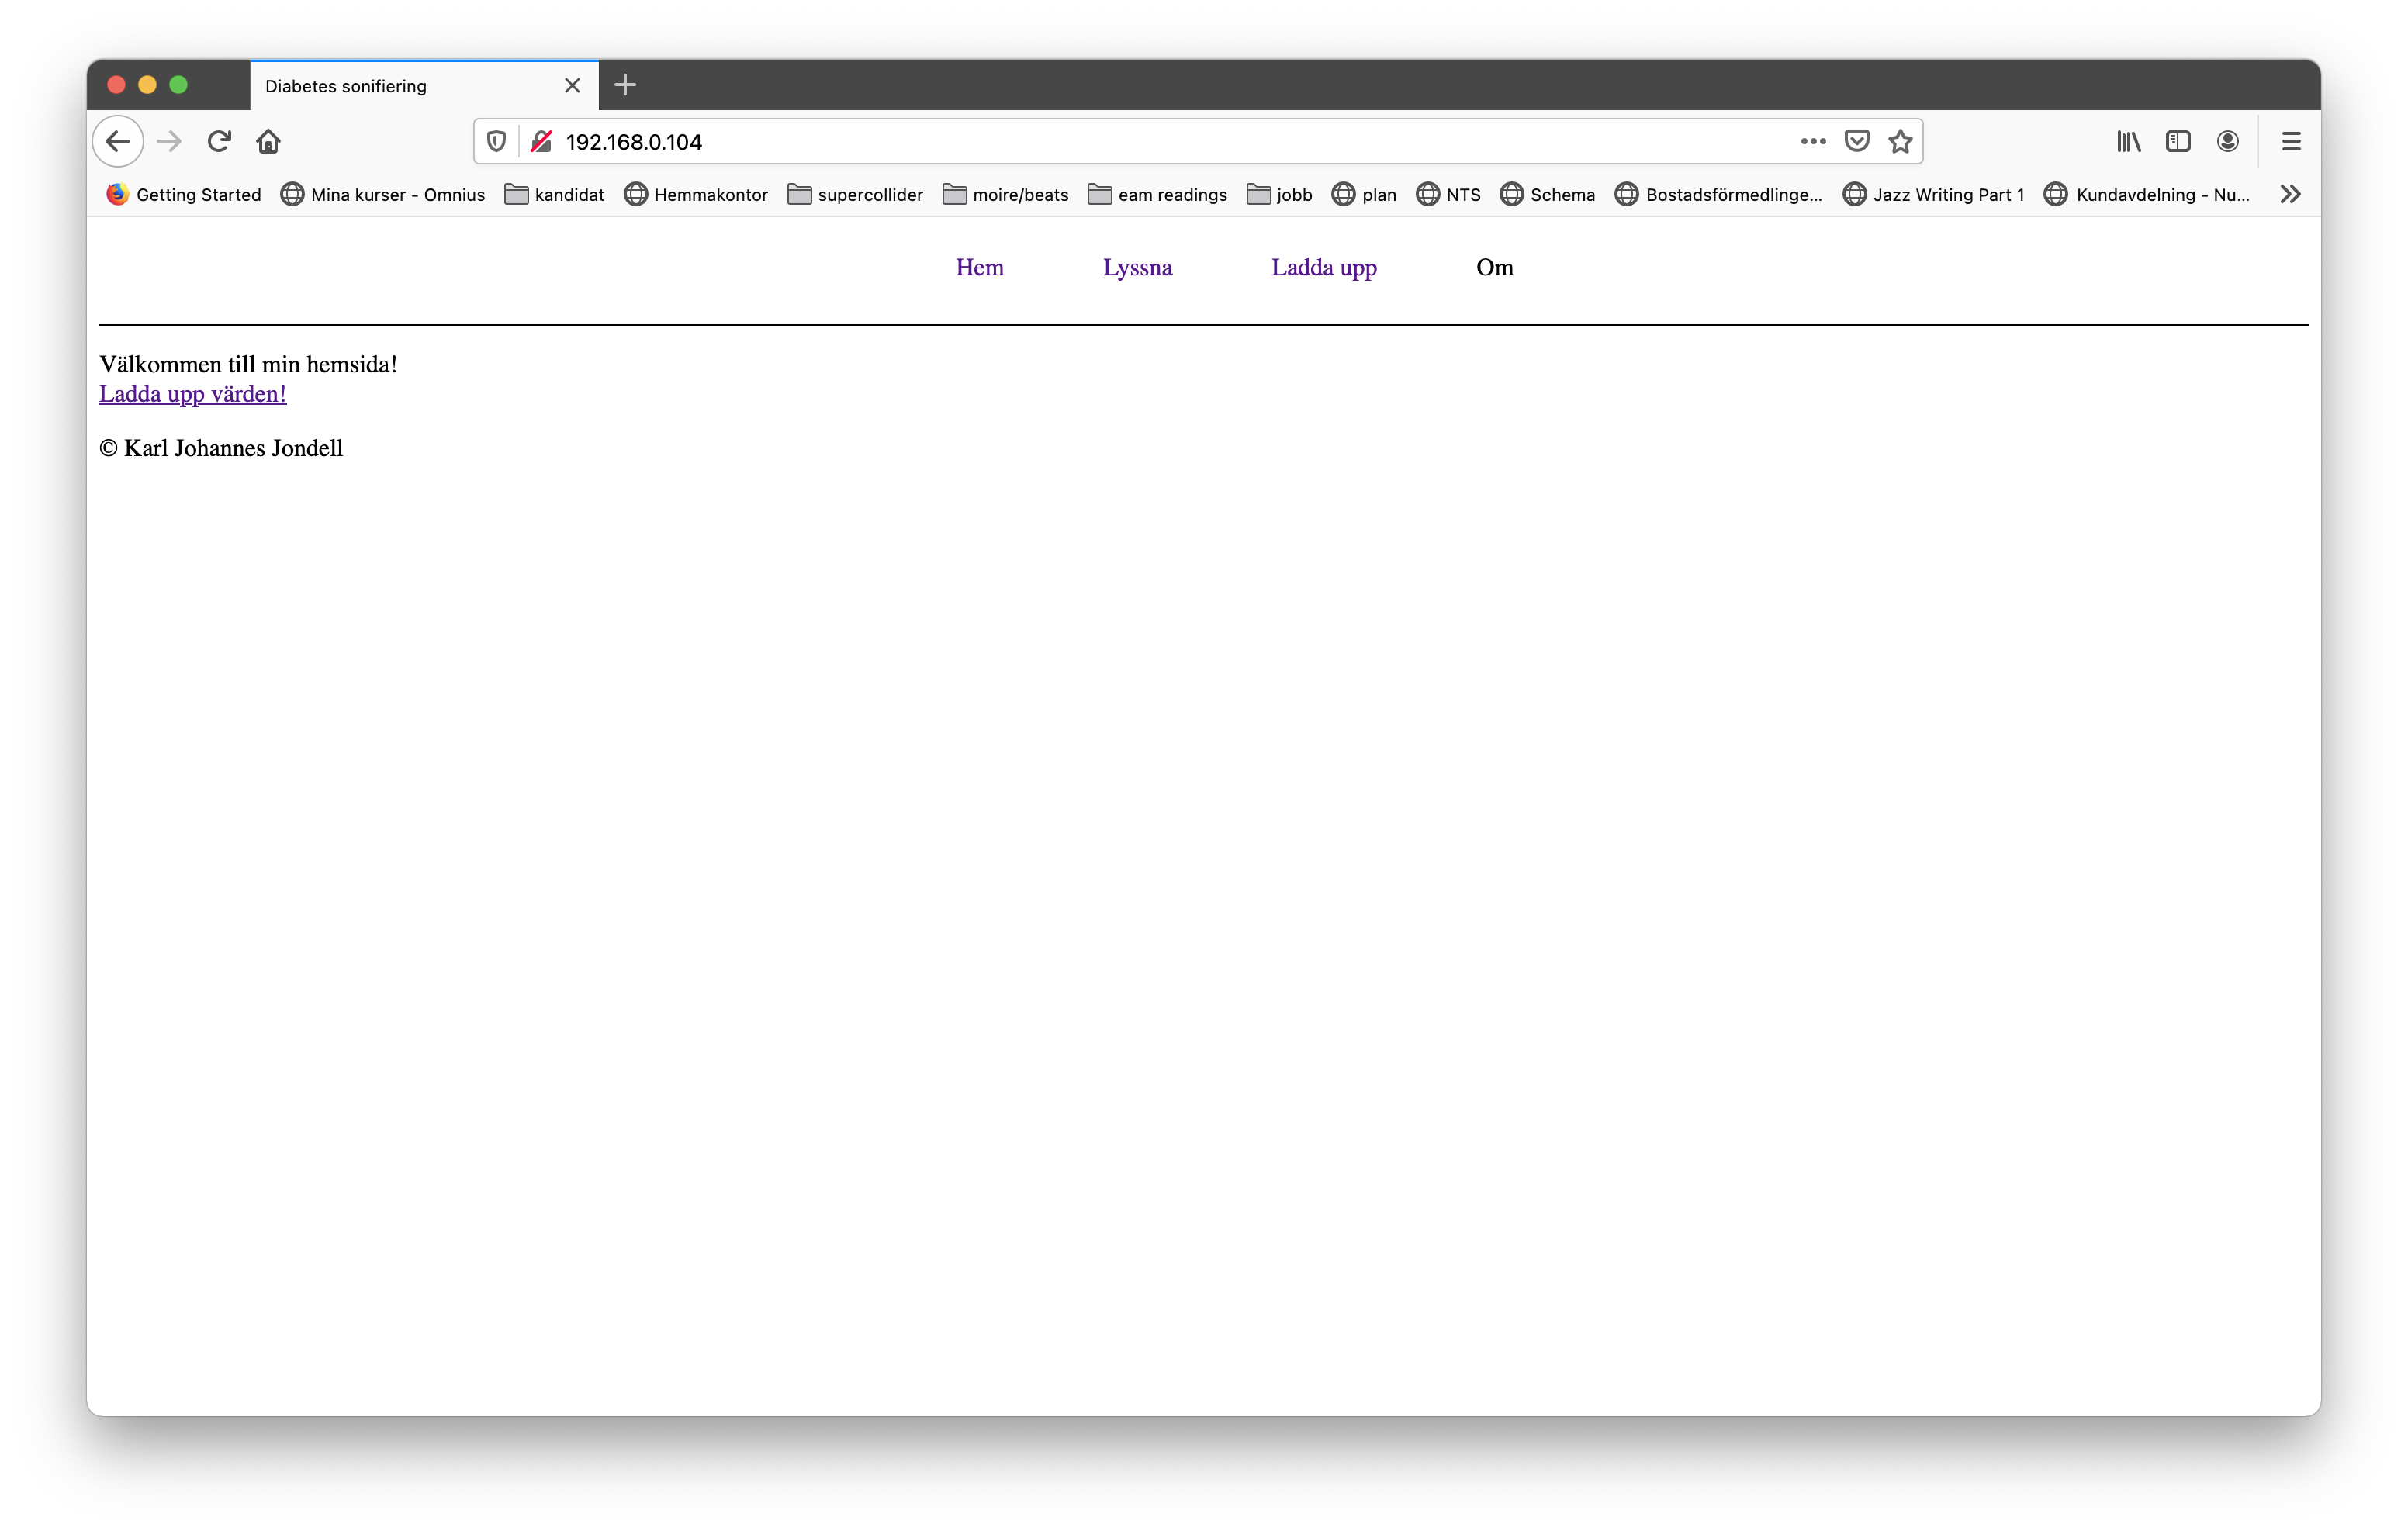
\includegraphics[width=\textwidth]{../media/hemsida.png}
\caption{Skärmdump av hemsida (\emph{temporär})}
\label{hemsida}
\end{figure*}

\subsection*{Webbplats}
\addcontentsline{toc}{subsection}{Webbplats}

Webbplatsen finns tillgänglig på domänen\footcite{jondell_radio_nodate}: \url{https://radiodiabetes.eu/}. I figur \ref{hemsida} ovan visas en skärmdump av webbplatsen tagen den... %TODO insert date....

Webbplats består av en s.k. \emph{\gls{frontend}} och en \emph{\gls{backend}}. Linux (Ubuntu 20.04)/Nginx/gunicorn \gls{stack}.
\subsubsection*{Front end}
\addcontentsline{toc}{subsubsection}{\emph{Front end}}
1. beskriv vad frontend är för något
2. beskriv tekniken (react.js)

\subsubsection*{Back end}
\addcontentsline{toc}{subsubsection}{\emph{Back end}}
1. beskriv vad backend är för något (API?) \gls{api}
2. flask, darkice/icecast också kanske? 

\subsection*{Tillvägagångssätt}
\addcontentsline{toc}{subsection}{Tillvägagångssätt}
Hur jag gjort/reflektioner/vad jag ändrat

\section*{Musiken}
\addcontentsline{toc}{section}{Musiken}


% Lager, eller vilka SynthDefar jag har:
% 1. GSM (drone, eller bas/fundament, eller pad...)
% 2. Sinusvågor och elektroniska störningsljud (arpeggio, rytmiska, sextondelar, tempo)
% 3. Wavetable (pad)
% 4. JLC bas? resonator hum ? andra ljud ? ?? ? ? 

De musikaliska funktioner jag har representerade är dels ett fundament eller grund som utgörs av ett 

%Den konstnärliga friheten. Hur pass mycket kontroll som överlåtes till \enquote{serien} (i detta fall blodsockervärdet). Behöver musiken gestalta, spegla, estetisera erfarenheten som diabetiker? Eller vara intresseväckande, tillgänglig, \enquote{relaterbar}? 

\subsection*{Rumslighet}
\addcontentsline{toc}{subsection}{Rumslighet}
Varje objekt ges en unik position i stereofältet, och på så sätt en plats i rummet i musiken. 

Presentationen av radioströmmen genom hemsidan som jag har utformat påverkar också den upplevda rumsligheten i musiken. 

Ett planerat konserttillfälle kommer att ske den 20e maj i Lilla Salen i Musikhögskolan. Då spelas ett utdrag ur radioströmmen upp, som den hörs i realtid. I och med de rådande restriktionerna så kommer ingen publik kunna närvara, utan konserten strömmas vidare till en publik i etern. Själva konserttillfället blir därför en sorts manifestation av radioströmmen i tid och rum. 


% TODO tempusformulering


\subsection*{Temporalitet}
\addcontentsline{toc}{subsection}{Temporalitet}
Den tidsmässiga uppfattningen av musiken. En 24/7 livestream av musiken (hur utgörs lyssnadet? formen? \emph{Slow as possible}, \emph{Longplayer} och liknande...)

\subsection*{Generativt}
\addcontentsline{toc}{subsection}{Generativt}
Musiken är generativ. Serialism?

\section*{Slutsatser}
\addcontentsline{toc}{section}{Slutsatser}
Lärdomar etc...

\subsection*{Utvecklingsmöjligheter}
\addcontentsline{toc}{subsection}{Utvecklingsmöjligheter}
För mig är detta endast startskottet på ett projekt som kan växa på alla sätt. Jag har byggt en infrastruktur till en installation som går att utveckla.

- Gästbok/lämna röstmeddelanden...
- Två strömmmar: kunna växla mellan dem för att möjliggöra enklare utveckling av SuperCollider-systemet (utan att det behöver stängas ned för underhåll).
- Möjligheten att spela upp binauralt
- Internationellaisera (översätt hemsida etc...)


%\end{multicols}

%\twocolumn
%\clearpage
\addcontentsline{toc}{section}{Referenser}
\printbibheading
\printbibliography[type=article,title={Artiklar},heading=subbibintoc]
\printbibliography[type=book,title={Böcker},heading=subbibintoc]
\printbibliography[type=online,title={Hemsidor},heading=subbibintoc]
\printbibliography[type=audio,title={Musik},heading=subbibintoc]
\printbibliography[type=misc,title={Radio},heading=subbibintoc]
\printbibliography[type=incollection,title={Samlingar},heading=subbibintoc]

\clearpage
\begin{appendices}
\printglossaries
\end{appendices}

\end{document}

